
\documentclass[12pt, titlepage]{article}

\usepackage[pdftex]{graphicx}
\usepackage{booktabs}
\usepackage{tabularx}
\usepackage{hyperref}
\usepackage{float}
\hypersetup{
    colorlinks,
    citecolor=black,
    filecolor=black,
    linkcolor=red,
    urlcolor=blue
}
\usepackage[round]{natbib}

\title{SE 3XA3: Development Plan\\Mari0}

\author{Team 9, Ninetendo
		\\ David Hobson - hobsondd
		\\ Jose Miguel Ballesteros - ballesjm
		\\ Jeff Pineda - pinedaj
}

\date{\today}

%% Comments

\usepackage{color}

\newif\ifcomments\commentstrue

\ifcomments
\newcommand{\authornote}[3]{\textcolor{#1}{[#3 ---#2]}}
\newcommand{\todo}[1]{\textcolor{red}{[TODO: #1]}}
\else
\newcommand{\authornote}[3]{}
\newcommand{\todo}[1]{}
\fi

\newcommand{\wss}[1]{\authornote{blue}{SS}{#1}}
\newcommand{\ds}[1]{\authornote{red}{DS}{#1}}
\newcommand{\mj}[1]{\authornote{red}{MSN}{#1}}
\newcommand{\cm}[1]{\authornote{red}{CM}{#1}}
\newcommand{\mh}[1]{\authornote{red}{MH}{#1}}

% team members should be added for each team, like the following
% all comments left by the TAs or the instructor should be addressed
% by a corresponding comment from the Team

\newcommand{\tm}[1]{\authornote{magenta}{Team}{#1}}


\begin{document}

\maketitle

\pagenumbering{roman}
\tableofcontents
\listoftables
\listoffigures

\begin{table}[bp]
\caption{\bf Revision History}
\begin{tabularx}{\textwidth}{p{3cm}p{2cm}X}
\toprule {\bf Date} & {\bf Version} & {\bf Notes}\\
\midrule
October 6, 2016 & 1.0 & Created Document, rough draft of section 1\\
October 11, 2016 & 1.1 & Added Problem Issues\\
October 11, 2016 & 1.2 & Finished Project Drivers and Non-Functional Requirements\\
November 28, 2016 & 1.3 & Updated Functional Requirements to be more aligned with project\\
December 5, 2016 & 1.4 & Removed some terminology and definitions\\
\bottomrule
\end{tabularx}
\end{table}

\newpage

\pagenumbering{arabic}

This document describes the requirements for Mari0  The template for the Software
Requirements Specification (SRS) is a subset of the Volere
template~\citep{RobertsonAndRobertson2012}.

\section{Project Drivers}

\subsection{The Purpose of the Project}
The purpose of this project is to recreate the game, Mari0, to allow the players 
to entertain themselves and alleviate their boredom. Mari0 is a combination of
Super Mario Bros. and Portal, challenging a player's platforming abilities and their
puzzle solving skills.

\subsection{The Stakeholders}

\subsubsection{The Client}
The client for the Mari0 project is the game publisher.

\subsubsection{The Customers}
The customers for this project are people interested in platforming and/or puzzle games.

\subsubsection{Other Stakeholders}
The other stakeholders for Mari0 are the game's developers and designers. Along with the client and the customers that are interested in playing games and puzzles.

\subsection{Mandated Constraints}
The constraints as mandated by our client are as follows:
\begin{itemize}
	\item Have each deliverable finished by the deadlines given in the course outline
	\item The game's physics will be handled by the Unity Game engine
	\item The product should be runnable on all operate systems
\end{itemize}

\subsection{Naming Conventions and Terminology}

\begin{table}
\caption{Terminology and Definition Table}
\begin{tabular}{l l}
\hline
Term			& Definition \\
\hline
Mario      		 & The character that the player portrays  \\
Portals      		 & Two connected portals that allow characters and projectiles to \\
			 & enter one and exit through the other, whilst maintaining physics \\
			 & properties such as velocity and acceleration \\
Goomba		 & Enemy character that is defeated after the player stomps on the top \\
			 & of its head	  \\
			 & the top of its head; leaves behind a shell that can be used as a projectile	\\
A.I.			 & Artificial Intelligence  \\
Lives			 & The amount of times the player can die before game over	\\
Question Block	 & Blocks found that when hit give the player coins or power ups	\\
\hline
\end{tabular}
\end{table}

\subsection{Relevant Facts and Assumptions}

The users of this game are the players, and despite Mari0 being derived from the games Super Mario Bros. and Portal, the mechanics and game knowledge that come from playing these games is not assumed. \\
It is also assumed that the user has a computer, a keyboard, and a mouse to play the game.

\section{Functional Requirements}

\subsection{The Scope of the Work and the Product}

\subsubsection{The Context of the Work}
The game design and interface will be simple and effective. The user will be able to provide input through their computers and will be able to receive the expected response, as shown in Figure \ref{fig:context}. For example, if the user presses the up button and expects to jump, the character on screen will provide a jumping animation for feedback.
\begin{figure}[h] %  figure placement: here, top, bottom, or page
   \centering
   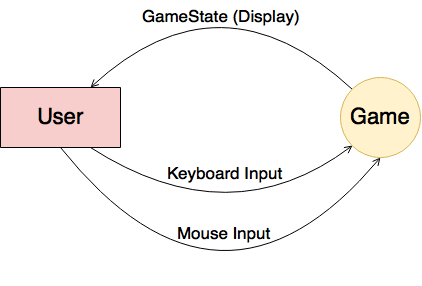
\includegraphics[width=3in]{Fig1} 
   \caption{Context Diagram of the gaming system}
   \label{fig:context}
\end{figure}

\subsubsection{Work Partitioning}
\begin{table}[H]
\caption{Work Partitioning}
\begin{tabular}{lll}
\hline
Event Name & Input/Output & Summary\\
\hline
Menu Change      	&  Keyboard(in)/Mouse(in)  & When the user selects a menu that they'd\\
& GameState (Out) & like to visit, the menu will display it   \\

Movement      		&  Keyboard(in)  & When the user presses a key to move\\  
& GameState (Out) & the character, the character will display \\
& & its movement animations   \\

Jumping		 &  Keyboard(in)  & When the user presses a key to jump\\  
& GameState (Out) & the character, the character will display \\
& & its jumping animations   \\

Portal Shooting	 &  Mouse(in)  & When the user clicks where and which\\  
& GameState (Out) & portal they'd like to shoot, the game \\
& & iwill display them accordingly   \\

Enemy Hits Player			 &  GameState(Out)  & When an enemy hits the character the \\  
& & game will display the defeat animation \\
& & and the game will reset with one less life   \\

Player Hits Enemy		 &  GameState(Out)  & When the character hits an enemy on the\\  
& &  right spot, the enemy will disappear \\

Scoring	 &  GameState(Out)  & When the character collects points,  \\  
& & the game's score display will increase \\

Pause	 &   Keyboard(in) & When the user presses the pause key, \\  
& GameState(Out)& the game will display the pause menu \\
\hline
\end{tabular}
\end{table}

\subsubsection{Individual Product Use Cases}

Use Case \#: 1\\
Name: Play Game\\
Trigger: The user selects to play a new game\\
Precondition: The game is in its main menu\\
Post Condition: The game begins\\
\\
\\
\\
Use Case \#: 2\\
Name: Help \\
Trigger: The user selects to view help options\\
Precondition: The game is in its main menu\\
Post Condition: The help menu displays\\
\\
Use Case \#: 3\\
Name: Character Moves\\
Trigger: The user presses a key to move their character in a certain direction\\
Precondition: The game is playing\\
Post Condition: The character will move in the corresponding direction\\
\\
Use Case \#: 4\\
Name: Portal gets fired\\
Trigger: The user places the mouse where they'd want a portal and clicks left or right for which portal they want\\
Precondition: The game is playing and the portal is in a plausible place\\
Post Condition: The portal will get formed\\
\\
Use Case \#: 5\\
Name: Pause\\
Trigger: The user presses the pause key\\
Precondition: The game is playing\\
Post Condition: The pause menu is shown\\

\subsection{Functional Requirements}
\begin{enumerate}
\item \textbf{The game will have a main menu with multiple options for the user.} \\
\underline{\textit{Rationale:}}  The game must feature a place to have all gameplay options organized before a new game begins\\
\underline{\textit{Fit criterion:}} Main menu is displayed upon running.\\

\item \textbf{The game will feature a help menu}.\\
\underline{\textit{Rationale:}} The game must have some sort of way of telling the user how to play the game.\\
\underline{\textit{Fit criterion:}} Help menu is displayed when selected\\

\item \textbf{The user will be able to pause the game.}\\
\underline{\textit{Rationale:}} The game must allow the user to pause gameplay so that they can take a break when needed\\
\underline{\textit{Fit criterion:}} Gameplay is paused and the game stops.\\

\item \textbf{The game will display the character's current state.}\\
\underline{\textit{Rationale:}} The user needs a method to track lives and score\\
\underline{\textit{Fit criterion:}} The game displays the character's current score\\

\item \textbf{The game will feature portal system.}\\
\underline{\textit{Rationale:}} The gameplay must feature a method to help the user escape difficult situations\\
\underline{\textit{Fit criterion:}} The user is able to select which portal they want and where they'd place it\\

\item \textbf{The user will be able to move their character.}\\
\underline{\textit{Rationale:}} The user must have a way to move their character around the screen\\
\underline{\textit{Fit criterion:}} The user is able to move the character to their desired location\\

\item \textbf{The user will be able to make their character jump.} \\
\underline{\textit{Rationale:}}The user must have a method to make their character escape obstacles\\
\underline{\textit{Fit criterion:}} The user is able to see their character jump as wanted\\

\item \textbf{The game will feature powers ups.}\\
\underline{\textit{Rationale:}} The game must allow for ways to help the user's character\\
\underline{\textit{Fit criterion:}} The user gets benefit from the power up\\

\item \textbf{The character will be able to collect coin.}\\
\underline{\textit{Rationale:}} The user needs ways to increase their character's score\\
\underline{\textit{Fit criterion:}} The game will increase score total when the character collects a coin  \\

\item \textbf{Enemies will defeat the character}\\
\underline{\textit{Rationale:}} The game uses this technique to add difficulty to the game\\
\underline{\textit{Fit criterion:}} The character will display the defeat animation when hit by an enemy\\

\item \textbf{Characters will be able to defeat enemies.}\\
\underline{\textit{Rationale:}} The game needs a method to defeat enemies\\
\underline{\textit{Fit criterion:}} Enemies will be defeated when hit by the character from the top\\

\item \textbf{The character may fall off the platforms.} \\
\underline{\textit{Rationale:}} The user's ability to control their character will add difficulty to the game\\
\underline{\textit{Fit criterion:}} Character will be beaten after a fall off screen\\

\item \textbf{The character will be able to increase their score.} \\
\underline{\textit{Rationale:}} The game needs a way to increase score to have different gameplay scenarios\\
\underline{\textit{Fit criterion:}} The character can increase score after beating an enemy or collecting a coin\\
\section{Non-functional Requirements}
The numbers to the left of each listed requirement indicates requirement number/label.
\end{enumerate}

\subsection{Look and Feel Requirements}
\begin{enumerate}
\setcounter{enumi}{15}
	\item The game will load the two dimensional level the player is currently on. The playable foreground should be composed of Mario, enemies, and a variety of bricks with different attributes that can serve as platforms to jump to and from. The background of the level will change depending on the where the level is located. If the level is outside, the background will consist of a blue sky with a few clouds, small hills, and small bushes. If the level is underground or in a castle, the background will be pure black with no additional aesthetics added.
	\item The interface displaying the player's number of lives remaining, the current level, coins earned, and the time remaining in a non-obtrusive manner.
\end{enumerate}

\subsection{Usability and Humanity Requirements}
\begin{enumerate}
\setcounter{enumi}{17}
	\item The game should be easy to learn for all player's, regardless of their experience with the Super Mario Bros., Portal, or other similar games.
	\item The game should be fun and entertaining.
\end{enumerate}

\subsection{Performance Requirements}
\begin{enumerate}
\setcounter{enumi}{19}
	\item The game's visuals should respond to all commands inputted by the user without a noticeable delay. This will ensure that the player feels in full control at all times.
\end{enumerate}

\subsection{Operational and Environmental Requirements}
\begin{enumerate}
\setcounter{enumi}{20}
	\item The game should be able to run on any laptop or desktop computer.
\end{enumerate}

\subsection{Maintainability and Support Requirements}
\begin{enumerate}
\setcounter{enumi}{21}
	\item The game should be able to execute on Windows, OSX, and Linux based machines.
\end{enumerate}

\subsection{Security Requirements}
\begin{enumerate}
\setcounter{enumi}{22}
	\item The game should not be able access or alter any information on the user's computer besides updating the player's saved game files.
\end{enumerate}

\subsection{Cultural Requirements}
\begin{enumerate}
\setcounter{enumi}{23}
	\item The game's written components, such as messages and menu options should be written in English.
	\item The game should not have any messages, images, or depictions of religious, political, or ethnic significance.
\end{enumerate}

\subsection{Legal Requirements}
\begin{enumerate}
\setcounter{enumi}{25}
	\item The game should be licensed under the Creative Commons by Non-Commercial Share-Alike 3.0 license. 
\end{enumerate}

\subsection{Health and Safety Requirements}
\begin{enumerate}
\setcounter{enumi}{26}
	\item The game should not have any triggers for epileptic seizures.
\end{enumerate}

\section{Project Issues}

\subsection{Open Issues}
Currently, there a no known major issues for the project, however as the implementation continues there may need to be changes and problems may start to occur. 
Here are the list of some current issues with the game that may need to be improved:
\begin{itemize}
\item Some old operating systems such as Windows XP and Windows 7 have difficulty running the game properly.
\item Lack of modding support.
\item Players run into problems accessing the save folders.
\item Players have trouble using the Love framework in order to run the game
\end{itemize}

\subsection{Off-the-Shelf Solutions}
A lot of the issues will be solved easily with the use of Unity, since it is professionally made for game developers, and it is accessible to many operating systems. Also players will not have to deal with the Love framework that is apart of the current Mari0 game, since the entire project will be created in Unity.
Furthermore, if there are any huge problems, the code that has created the current game can be slightly modified to fit with Unity and will be essentially used as a prototype. In addition, Unity has it's own physics engine that will be a huge help in creating the environment for the game, instead of creating the entire game environment from scratch.
It may also help to look into other successful Unity games to see how things have been implemented, some platforming games may give us insight into how to make sure the physics works best for our final product. 

\subsection{New Problems}
New problems have yet to arise in the implementation. However, using Unity may add more problems in how things will be ran on certain systems if we would like to port the game to a mobile device or a console system. Overall, no new problems are expected to rise as a result of this project.

\subsection{Tasks}
Tasks are listed and numbered below.
\begin{enumerate}
\item Structures - Create class hierarchies and main game objects.
\item Overall Mechanics - Getting the character moving between two portals and interacting with environment
\item Level Design - Creating levels that the user can play and the character can be placed into.
\item Interfaces - Main programming interfaces such as Menu, Game Over, and Pause Screens.
\item Graphics and Sound - Main graphics, music and animation for the game.
\item Improvements - Adding different aspects of the game such as newer levels or different mechanics.
\end{enumerate}

\subsection{Migration to the New Product}
Since we are creating the same product, there is no migration to a newer product at this time.

\subsection{Risks}
Overall, risks are few and far between when it comes to recreating Mari0, but there are some risks that we would like to minimize. Flashing colours on the screen may trigger epileptic seizures for some users. Also, if the game is not optimized well, overheating of the system may damage users systems or cause minor burns. Although the chances of these problems arising are extremely low, they will be kept in mind when creating the final product.

\subsection{Costs}
Currently there are no costs associated with this project.

\subsection{User Documentation and Training}
User Documentation will be created as per the SFWR 3XA3 guidelines. Training/Tutorial will be implemented into the game through screen shots or a small in game user manual.

\subsection{Waiting Room}
There are currently no requirements or problems that have not been met or solved. This section will be updated as needed.

\subsection{Ideas for Solutions}
There are currently no ideas for solutions and no overall plan for these solutions. This section will be updated as needed.

\bibliographystyle{plainnat}

\bibliography{SRS}

\newpage

\section{Appendix}

This section has been added to the Volere template.  This is where you can place
additional information.

\subsection{Symbolic Parameters}

The definition of the requirements will likely call for SYMBOLIC\_CONSTANTS.
Their values are defined in this section for easy maintenance.
\end{document}